\documentclass[tikz,border=2pt]{standalone}
\usepackage{amsmath,amssymb}
\usepackage{pgfplots}
\pgfplotsset{compat=1.18}
\usetikzlibrary{arrows.meta}
\begin{document}
% Exponential premium of an exponential loss with rate lambda = 1: Pi_alpha = alpha^{-1} log[1/(1-alpha)]
% starts at E[X] = 1, follows E[X] + alpha Var(X)/2 = 1 + alpha/2 near 0, and explodes as alpha -> lambda = 1.
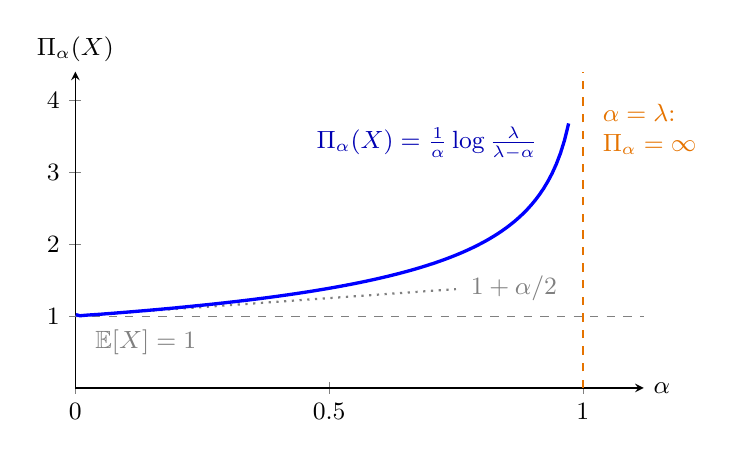
\begin{tikzpicture}[font=\small, >={Latex[length=2mm]}]
  \begin{axis}[
    axis lines=left, xmin=0, xmax=1.12, ymin=0, ymax=4.4,
    xtick={0,0.5,1}, ytick={1,2,3,4},
    xlabel={$\alpha$}, ylabel={$\Pi_\alpha(X)$},
    xlabel style={at={(axis description cs:1,0)}, anchor=west},
    ylabel style={rotate=-90, at={(axis description cs:0,1)}, anchor=south},
    width=8.8cm, height=5.6cm, clip=false
    ]
    \draw[gray, thin, dashed] (axis cs:0,1) -- (axis cs:1.12,1);
    \node[gray, anchor=north west] at (axis cs:0.02,0.95) {$\mathbb E[X]=1$};
    \addplot[gray, thick, dotted, domain=0:0.75, samples=2] {1+x/2};
    \node[gray, anchor=west] at (axis cs:0.76,1.38) {$1+\alpha/2$};
    \draw[orange!90!black, thick, dashed] (axis cs:1,0) -- (axis cs:1,4.4);
    \addplot[blue, very thick, domain=0.001:0.972, samples=120] {-ln(1-x)/x};
    \node[blue!70!black, anchor=east] at (axis cs:0.93,3.4) {$\Pi_\alpha(X)=\frac{1}{\alpha}\log\frac{\lambda}{\lambda-\alpha}$};
    \node[orange!90!black, anchor=west, align=left] at (axis cs:1.02,3.6) {$\alpha=\lambda$:\\$\Pi_\alpha=\infty$};
  \end{axis}
\end{tikzpicture}
\end{document}
